\documentclass{beamer}

\usepackage[utf8x]{inputenc} %arregla tema tildes y ñ
\usepackage[activeacute,spanish]{babel}
\usepackage{tikz}
\usepackage{wrapfig} % para meter fotitos volando por ahí
\usepackage[rflt]{floatflt}
\usepackage{graphicx}
\usepackage{subfigure}

\usetikzlibrary{arrows,shapes,arrows,chains,matrix}
%\usepackage[pdftex]{color}

%Tema
\usetheme{Warsaw}
%\usetheme{Berlin}


%\tikzstyle{blockPeque} = [rectangle, draw, thick,draw=gray!80,fill=gray!20,
%text width=80px, text centered, rounded corners, minimum height=13px,node distance = 3cm]

%Portada
\title{RF$^{2}$ - Recarga Fácil por Radio Frecuencia}
\author{Daniel Aicardi, Melina Rabinovich, Edgardo Vaz} 
\institute{
	Tutores: Ing. Juan Pablo Oliver, Ing. Andrés Aguirre\\

\bigskip
\bigskip
	Facultad de Ingeniería - UdelaR\\
	
	\bigskip
	
\includegraphics[scale=.2]{Imagenes/logos.jpg} \\%remove this line if no logo.
}

\date{\today}

\begin{document}

%Portada
\begin{frame}[plain]
	\titlepage
\end{frame} 


%\begin{frame}\frametitle{Esquema de la presentación}
%	\scriptsize 
%	\tableofcontents
%\end{frame}


%%\section{Introducción}
%\subsection{Sistema de Transporte}
\begin{frame}
	\frametitle{Sistema de transporte:}
	\begin{itemize}
		\item el pasajero usa su tarjeta como método de pago
		
		\bigskip
		\item dispositivo lector a bordo que debita viajes

		\bigskip
		\item recargar tarjetas

		\bigskip
		\item sistema de gestión de negocios (servidores, seguridad, puntos de venta)
	\end{itemize}
\end{frame}

\begin{frame}
	\frametitle{Sistema al día de hoy}
	
%	Al día de hoy:
	\begin{itemize}
		\item mundo PC
		
		\bigskip		
		\item puntos de venta concentrados

		\bigskip
		\item pago no desacoplado de la recarga

		\bigskip
		\item no está pensado 24/7		
	\end{itemize}
\end{frame}

\begin{frame}
	\frametitle{Sistema alternativo}
	
%	Alternativa:
	\begin{itemize}
		\item mundo sistemas embebidos

		\bigskip
		\item puntos de venta bien distribuídos

		\bigskip
		\item pago desacoplado de la recarga

		\bigskip
		\item 24/7		
	\end{itemize}
\end{frame}

\begin{frame}
	\frametitle{Descripción general del sistema de transporte}
	\begin{center}	
		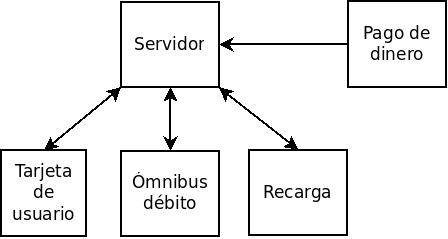
\includegraphics[scale=.5]{Imagenes/sistrans.jpg}
	\end{center}
\end{frame}

\begin{frame}
	\frametitle{Parte a implementar del sistema de transporte}
	\begin{center}
		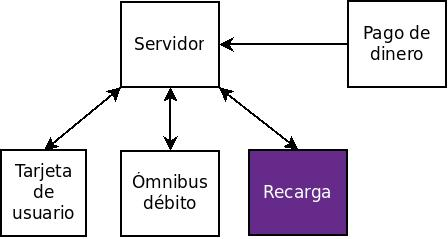
\includegraphics[scale=.5]{Imagenes/sistrans1.jpg}
	\end{center}
\end{frame}

\begin{frame}
	\frametitle{Parte a implementar del sistema de transporte}
	\begin{center}
		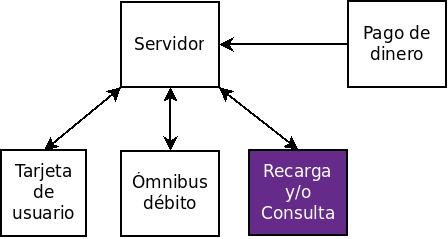
\includegraphics[scale=.5]{Imagenes/sistrans2.jpg}
	\end{center}
\end{frame}

%\section{Proyecto RF$^{2}$}
\begin{frame}
	\frametitle{Objetivos}
		\begin{block}{Objetivo principal}		
			Diseño y fabricación de un prototipo para recargar y consultar tarjetas RFID
		\end{block}

		\bigskip		
		Características principales del prototipo:
		\begin{itemize}			
			\item autónomo

			\bigskip
			\item seguro

			\bigskip
			\item bajo costo, consumo y mantenimiento
	
%			\bigskip
%			\item bajo consumo

%			\bigskip
%			\item bajo mantenimiento
		\end{itemize}

\end{frame}

%%\section{Hardware}
\begin{frame}
	\frametitle{Descripción del prototipo}
	\begin{itemize}
		\item sistema basado en un microprocesador (SBC)

		\bigskip
		\item lector/escritor de tarjetas RFID (antena)

		\bigskip
		\item lector/escritor de tarjetas de contacto (SAM)

		\bigskip
		\item interfaz de usuario
	\end{itemize}
\end{frame}

\begin{frame}
	\frametitle{Antecedentes}
	\begin{itemize}
		\item existen antecedentes de todas las partes

		\bigskip
		\item lectores/escritores de tarjetas RFID y de contacto orientados a PC 

		\bigskip
		\item OpenPCD - hardware y software abierto

		\bigskip
		\item AFE - dispositivo autónomo hecho en IM
	\end{itemize}	
\end{frame}

\begin{frame}
	\frametitle{Elección de arquitecturas}
	\begin{itemize}
		\item varias alternativas, muchas similares entre sí

		\bigskip
		\item las dos más factibles
	\end{itemize}
	\textcolor{red}{acá van imágenes de las 2 arq!!!}
	
\end{frame}

\begin{frame}
	\frametitle{Arquitectura, con OpenPCD vs. prototipo RF$^{2}$}
	\begin{center}
		\scalebox{0.8}{
		\begin{tabular}{c|c}
			OpenPCD & RF$^{2}$ \\ \hline
			dispara los costos & costos razonables\\
			dispositivo orientado a PC & dispositivo autónomo\\
			arquitectura similar al AFE & -\\
			- & diseño del lector/escritor RFID desde cero!!
		\end{tabular}}	
	\end{center}
\end{frame}

\begin{frame}
	\frametitle{Arquitectura definida}
	\begin{center}
		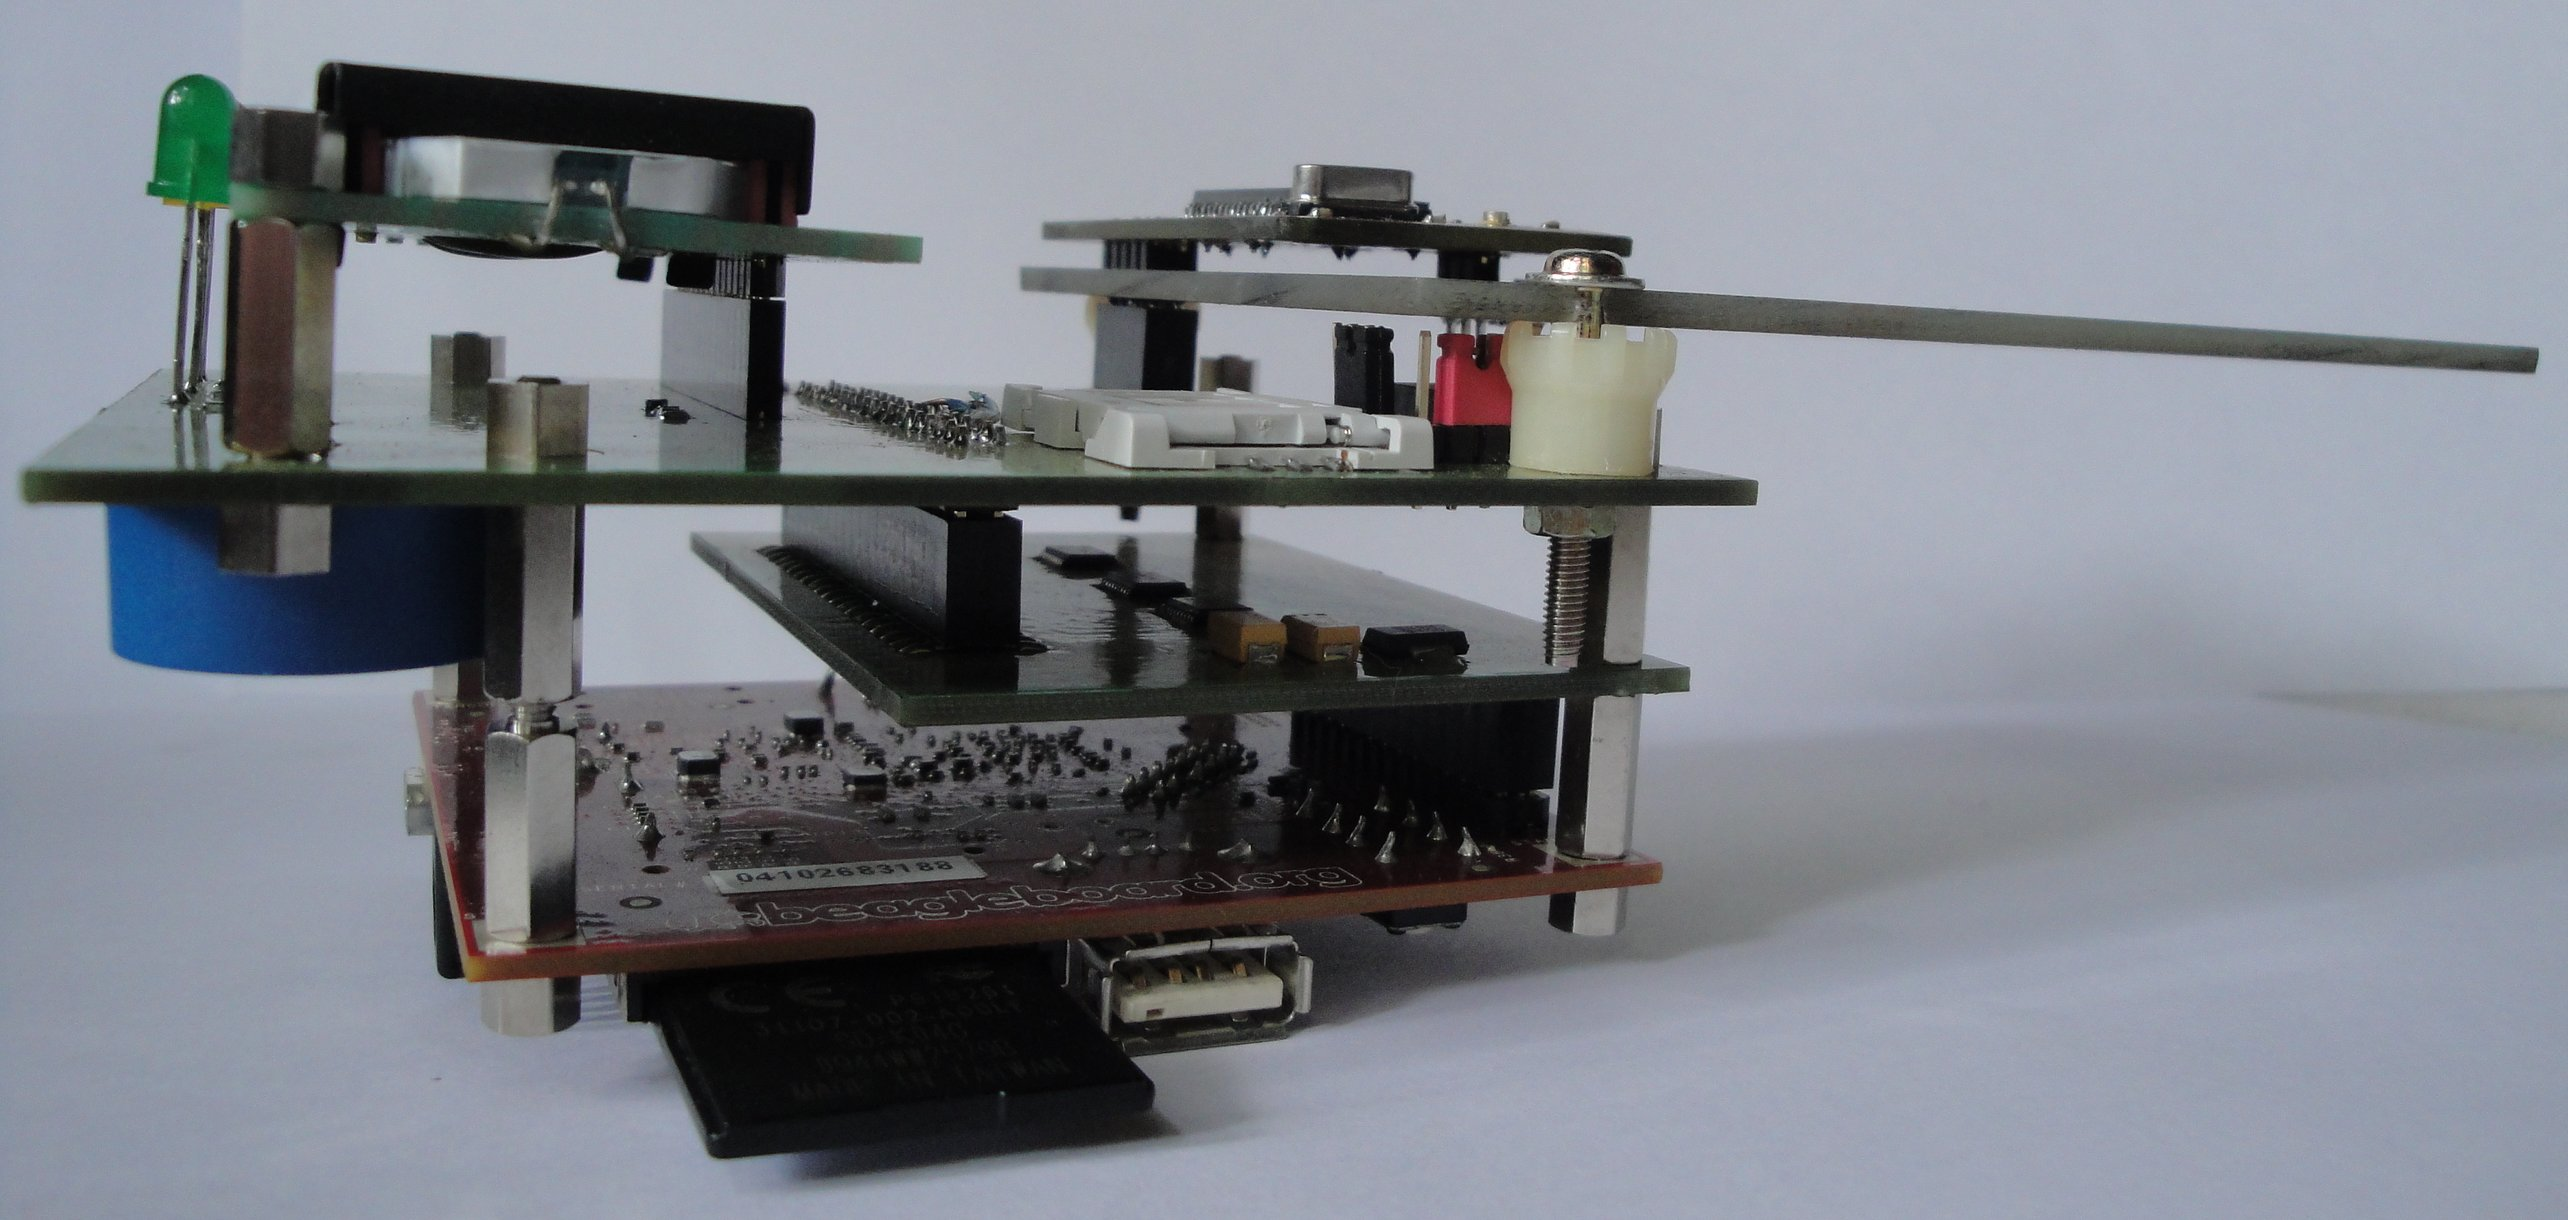
\includegraphics[scale=.12]{Imagenes/prototipo_s.jpg}
	\end{center}
\end{frame}


\begin{frame}
	\frametitle{Arquitectura definida}
	\begin{center}
		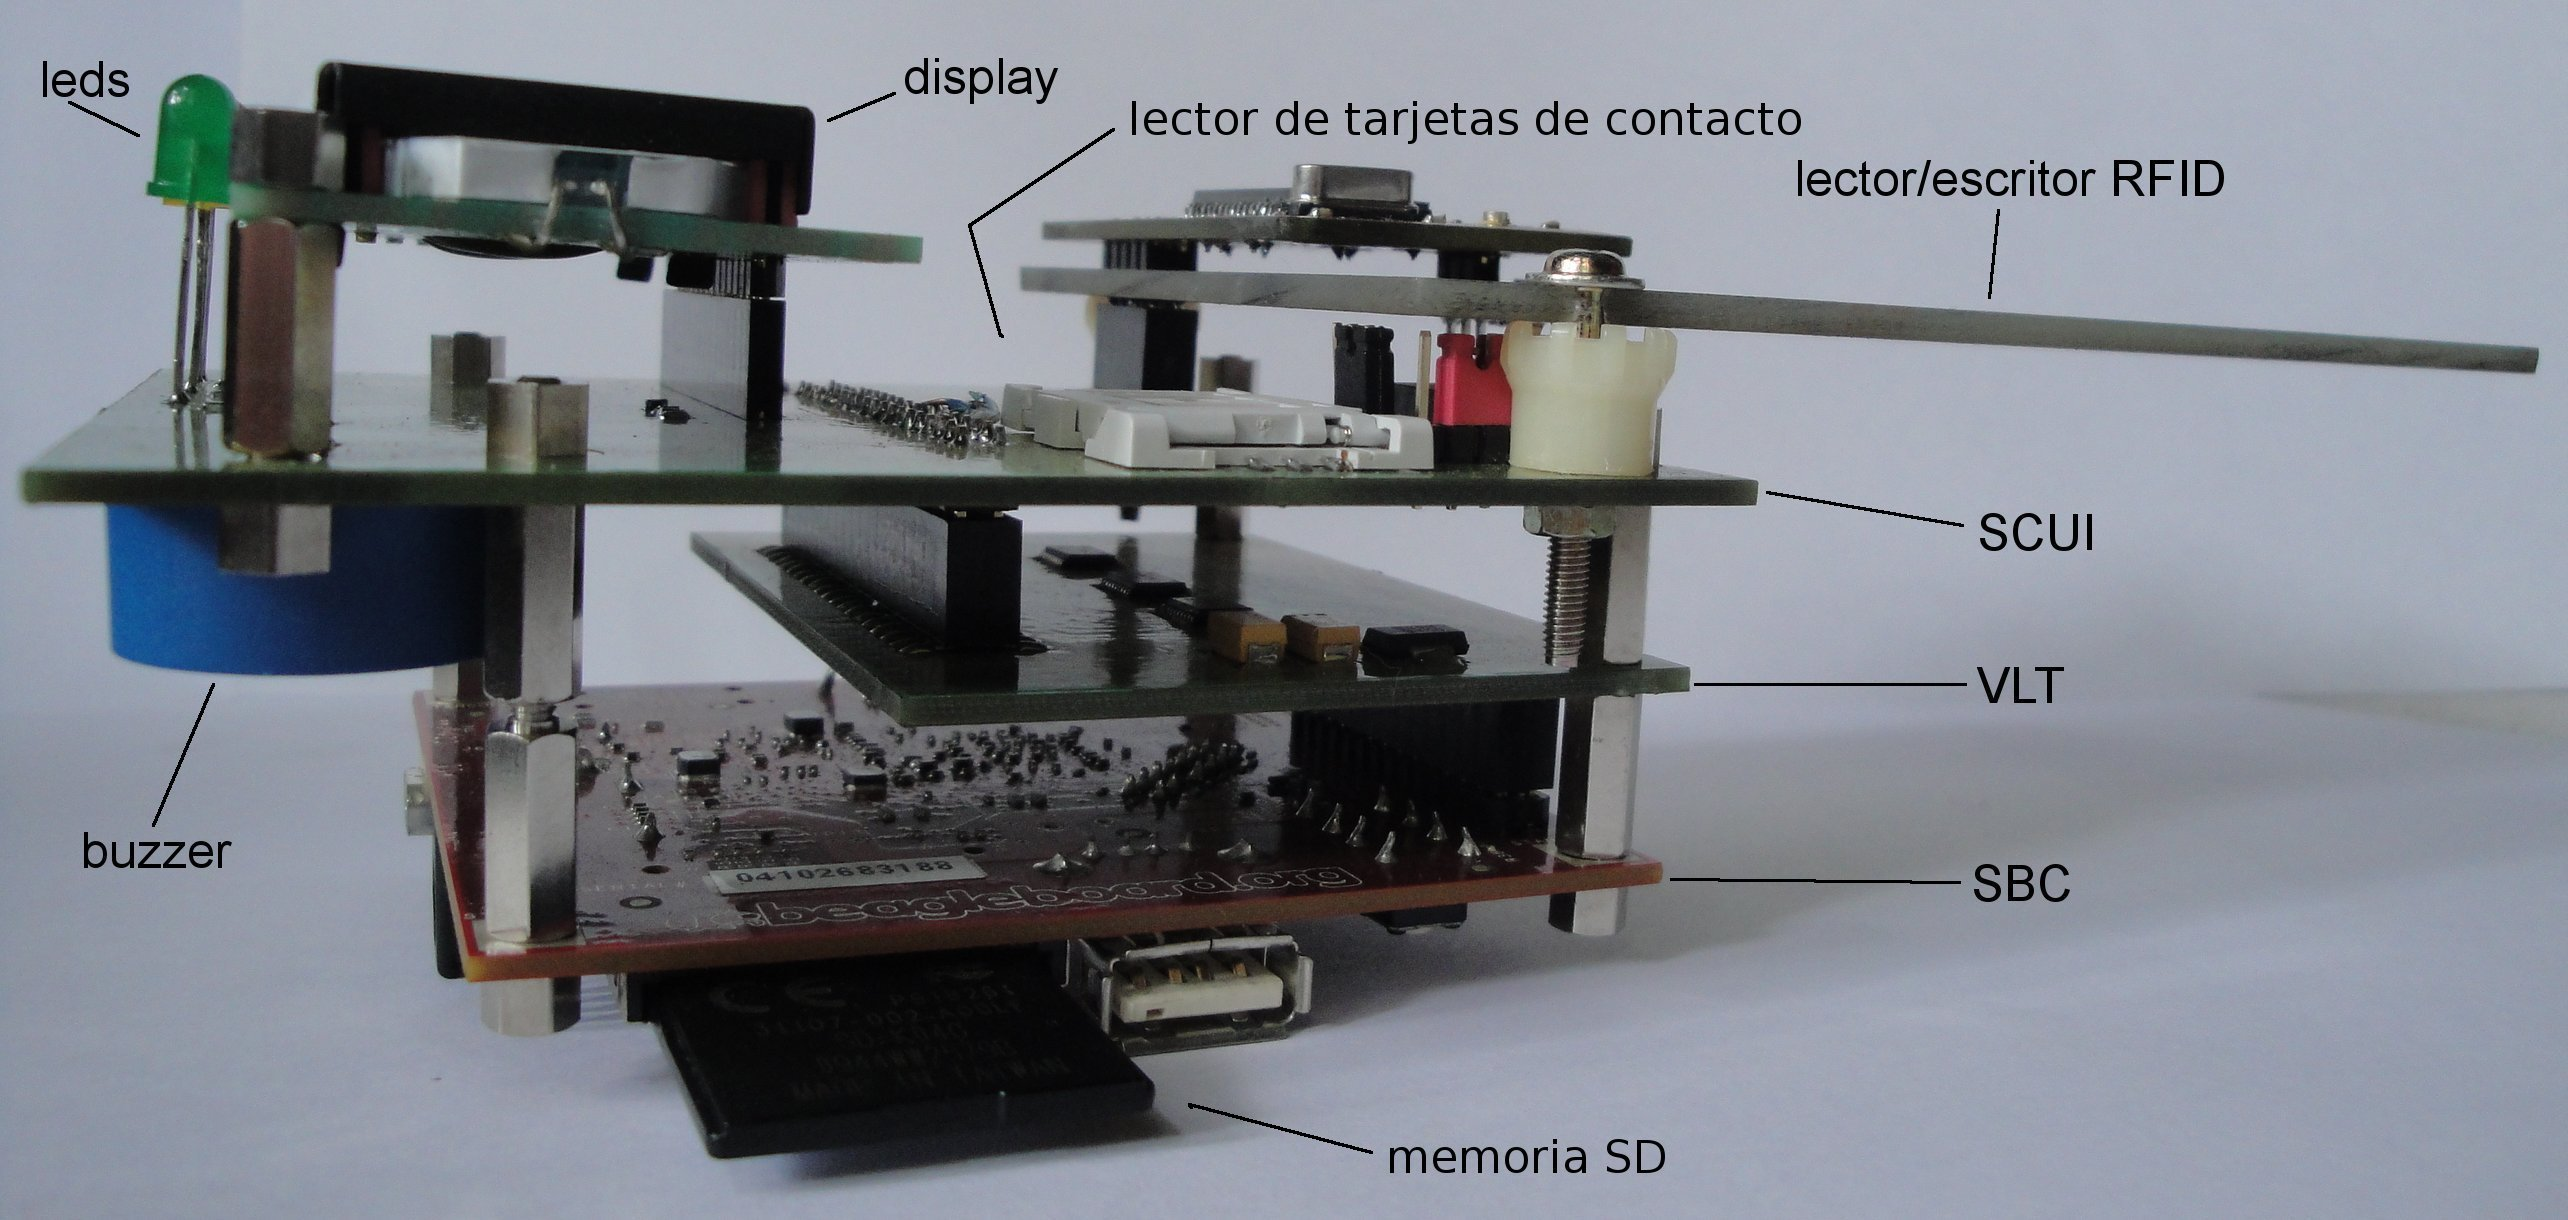
\includegraphics[scale=.12]{Imagenes/prototipo_s_nombres.jpg}
	\end{center}
\end{frame}

\begin{frame}
	\frametitle{SBC}
	Beagleboard:
	\begin{figure}
		\centering		
  		\subfigure{
	  		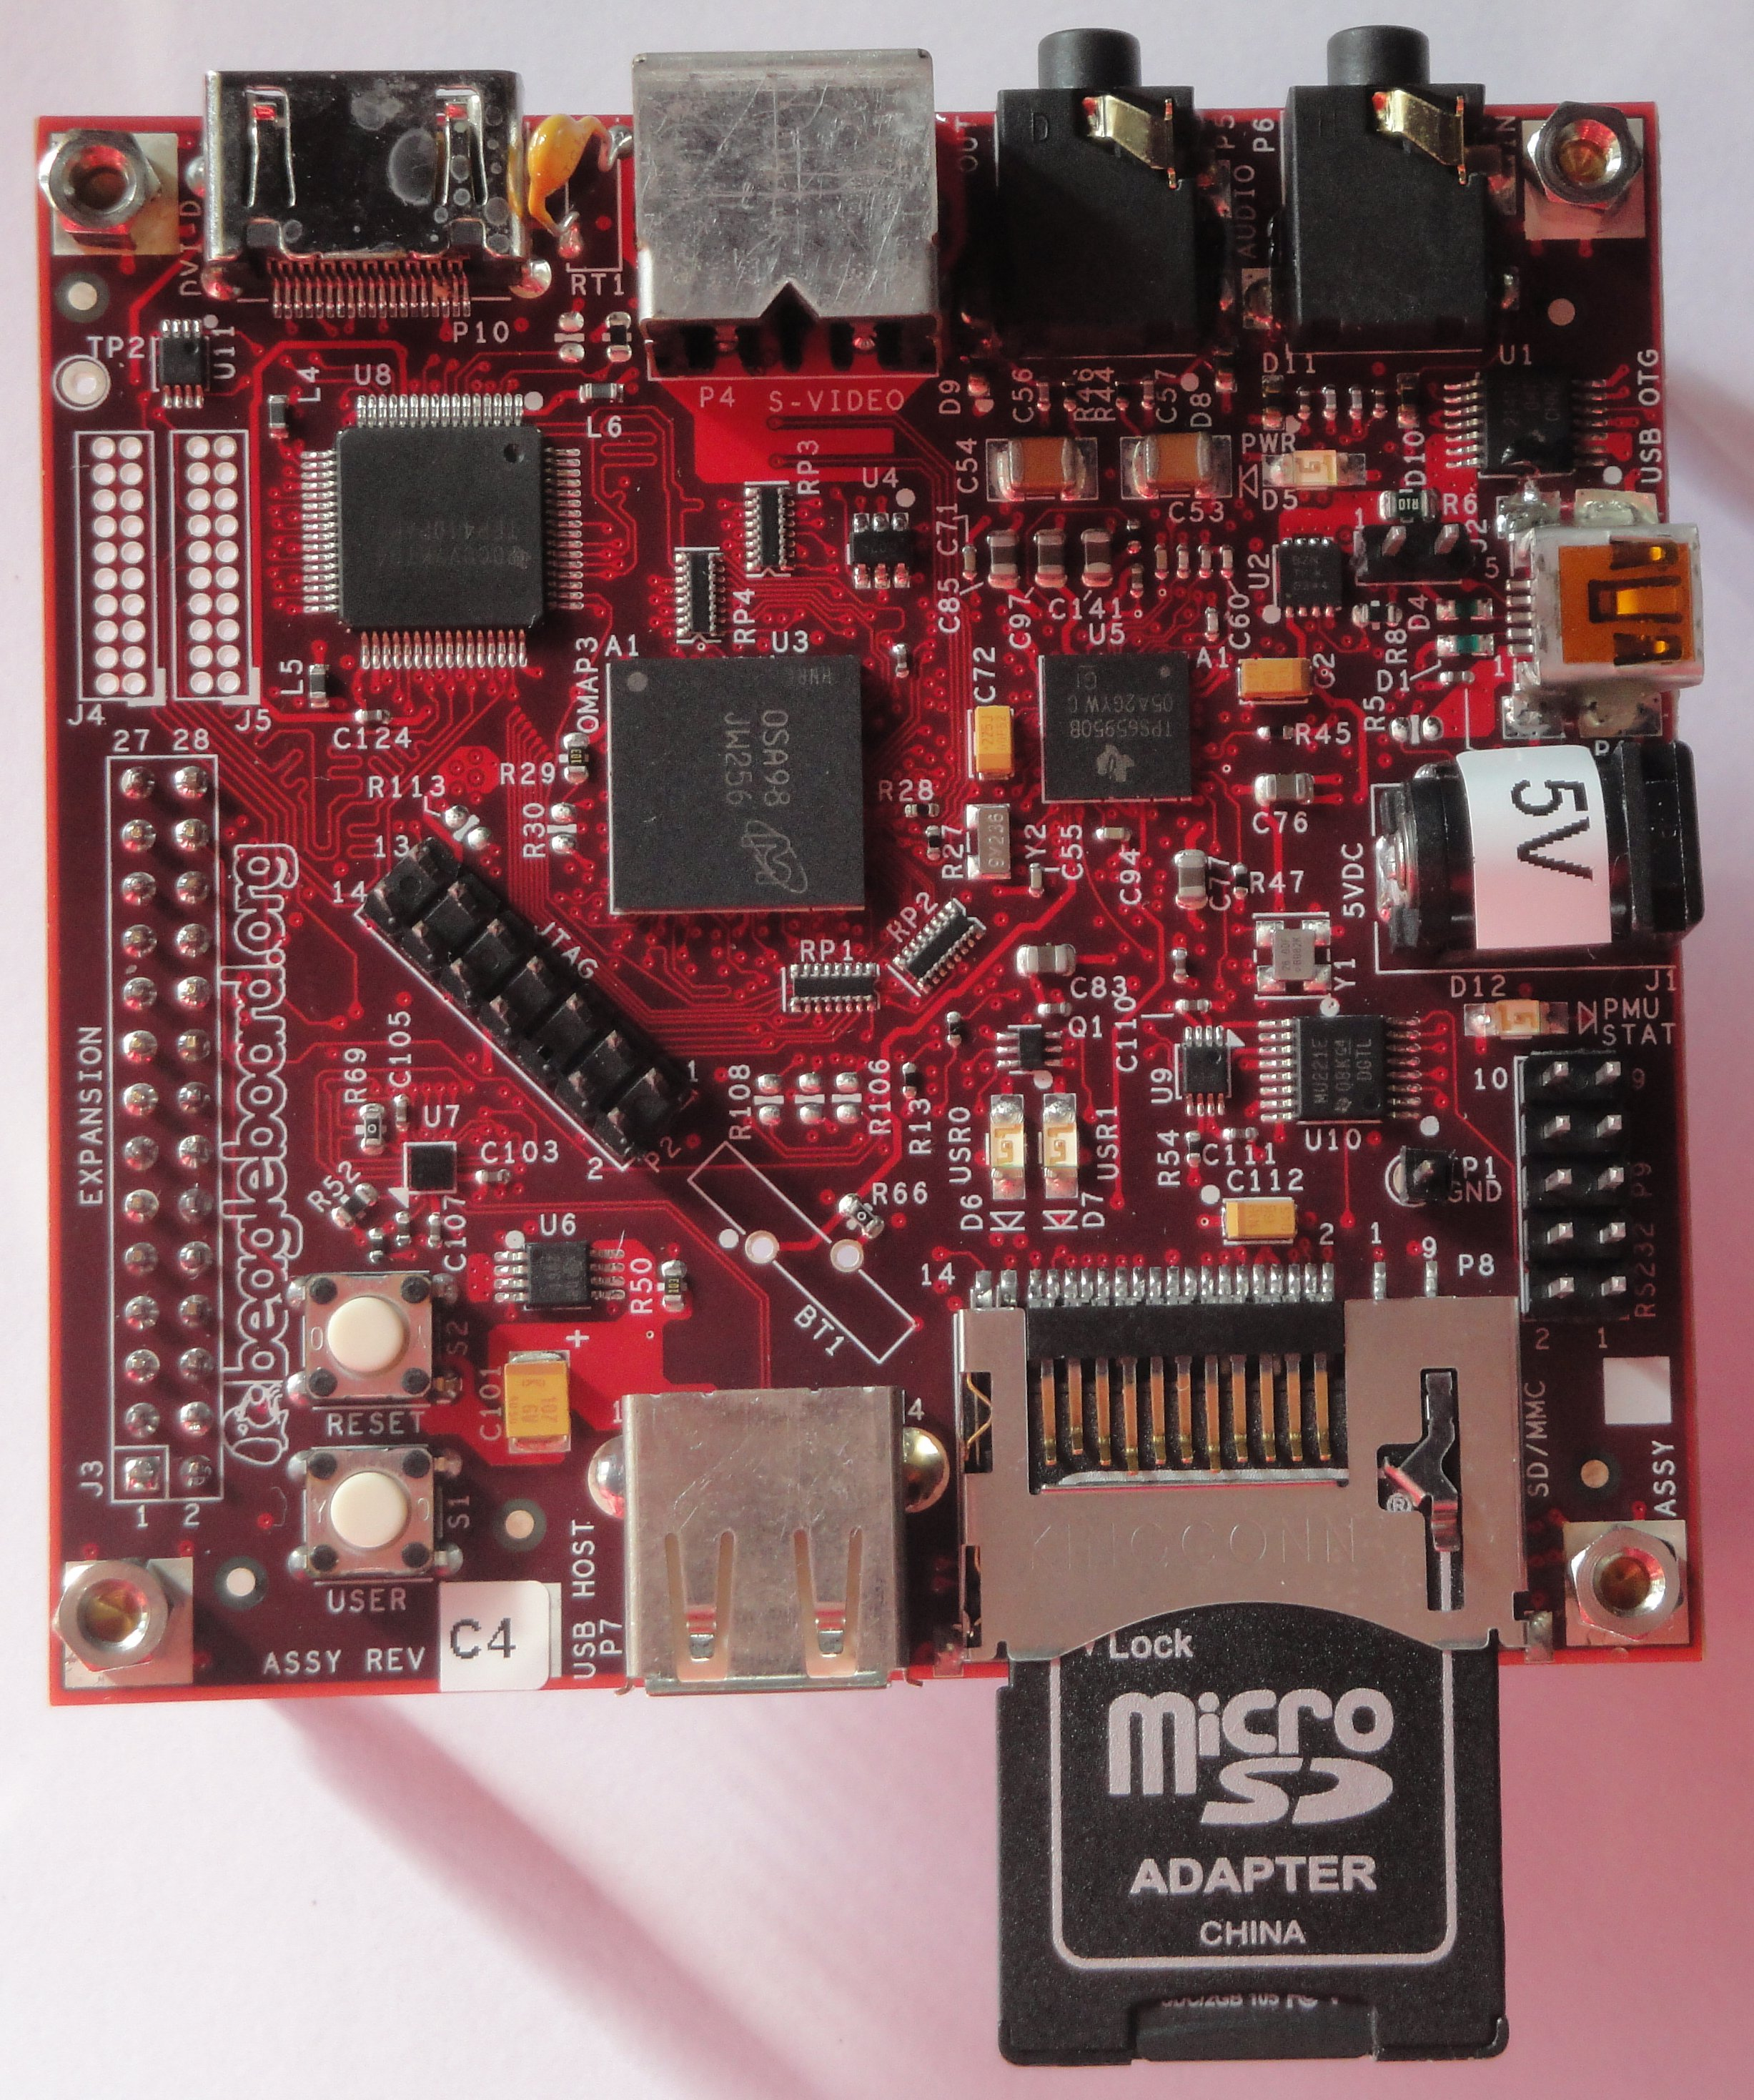
\includegraphics[scale=.03]{Imagenes/SBC_f.jpg} } 
	  	\subfigure{
	  		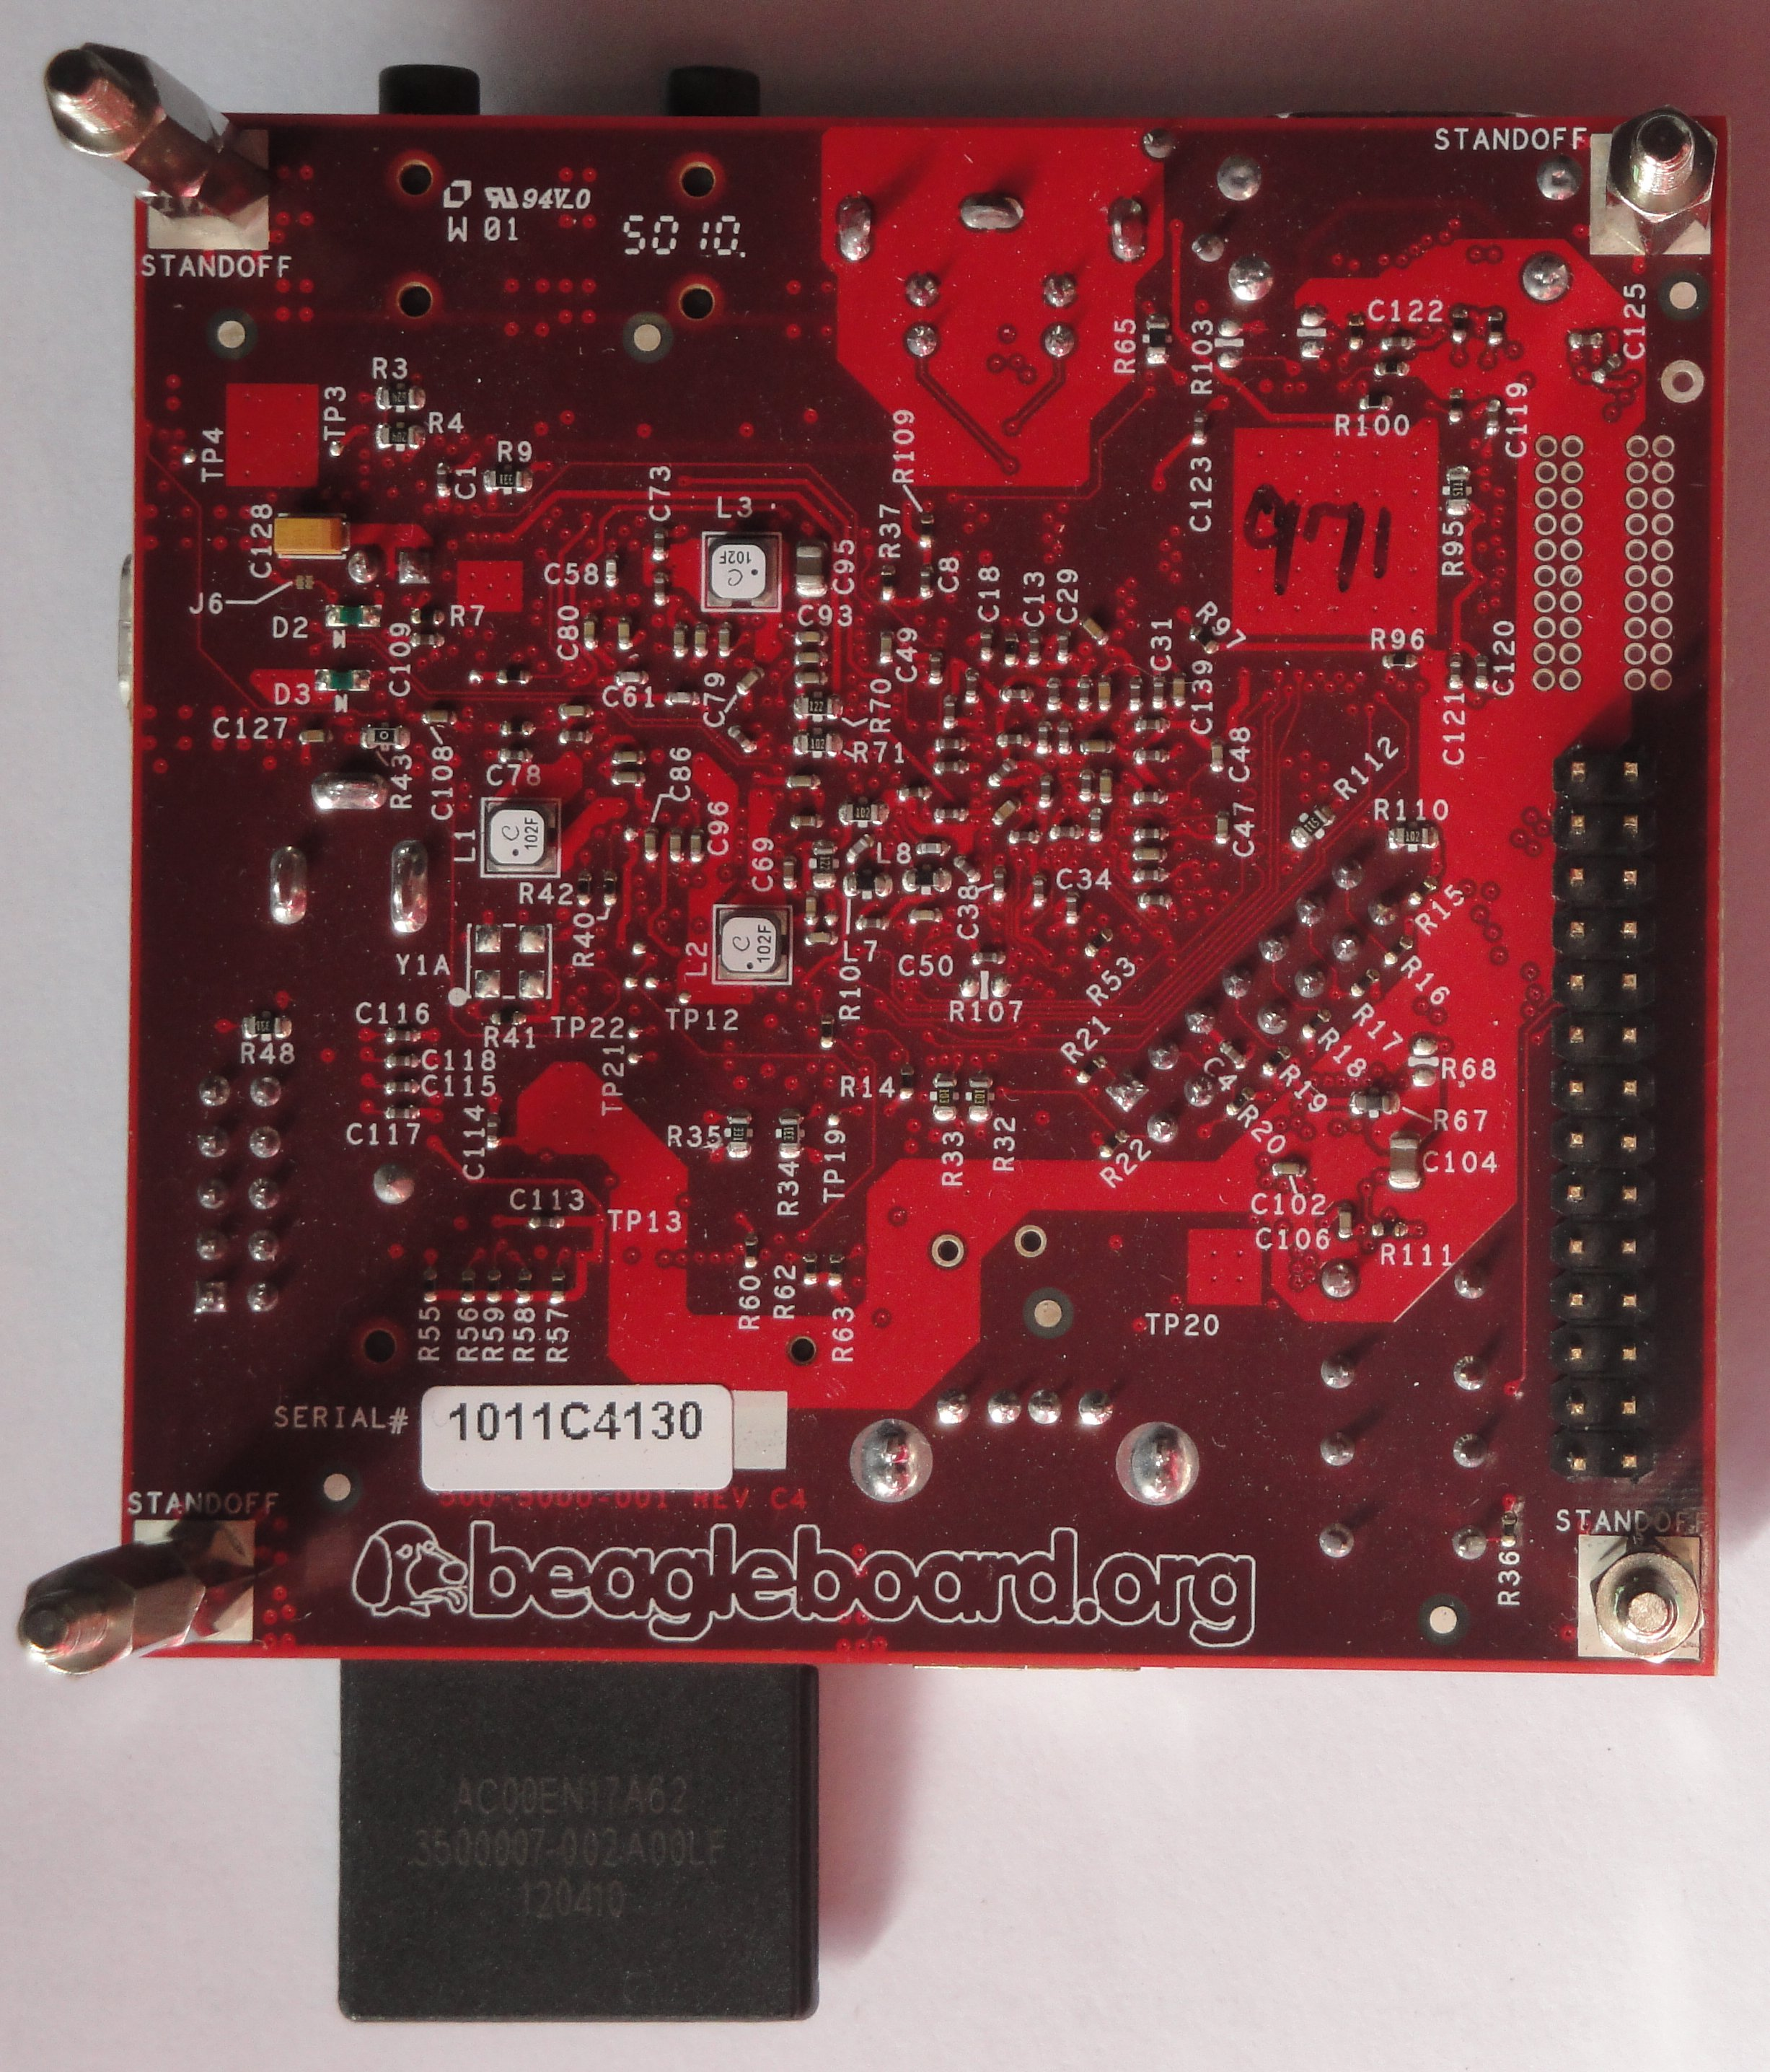
\includegraphics[scale=.03]{Imagenes/SBC_b.jpg} }
	\end{figure}

	\begin{itemize}
		\item es el sistema basado en un microprocesador

		\bigskip
		\item se compró

		\bigskip
		\item ejecuta el sistema operativo
	\end{itemize}
\end{frame}

\begin{frame}
	\frametitle{SCUI}
	Lector de tarjetas de contacto e interfaz de usuario:
	\begin{figure}
		\subfigure{
  			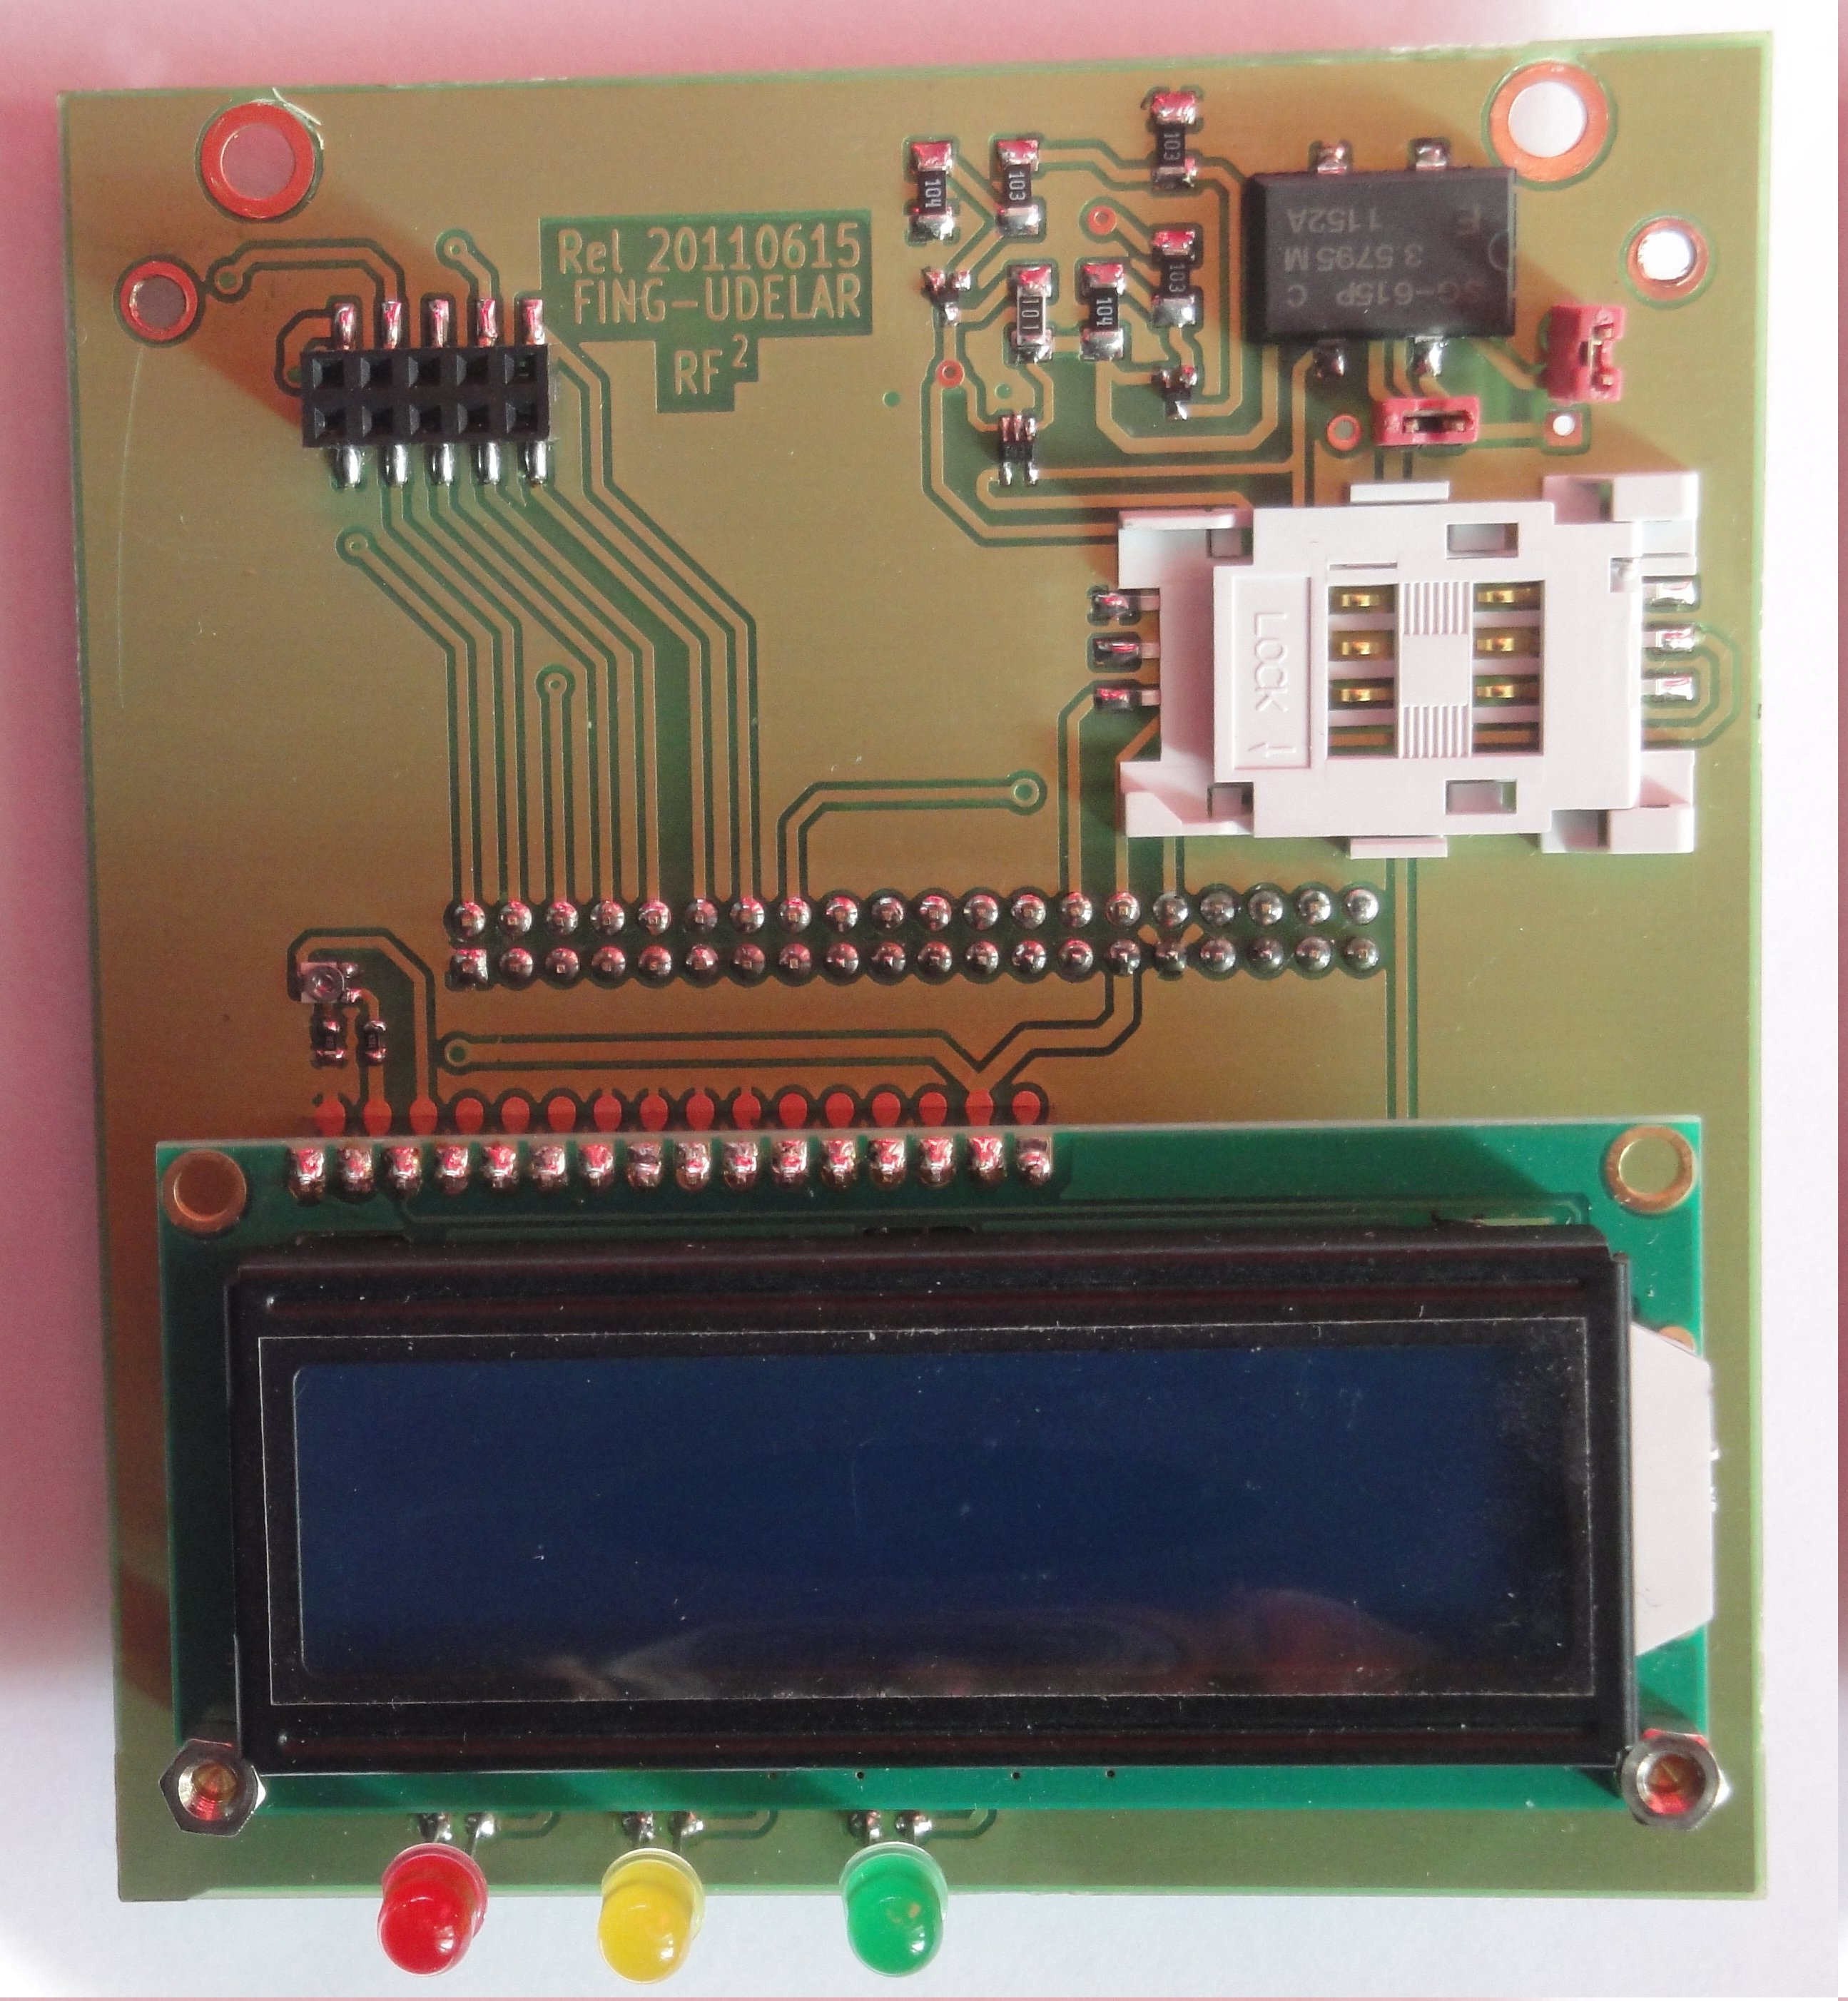
\includegraphics[scale=.03]{Imagenes/SCUI_f.jpg} } 
		\subfigure{ 
			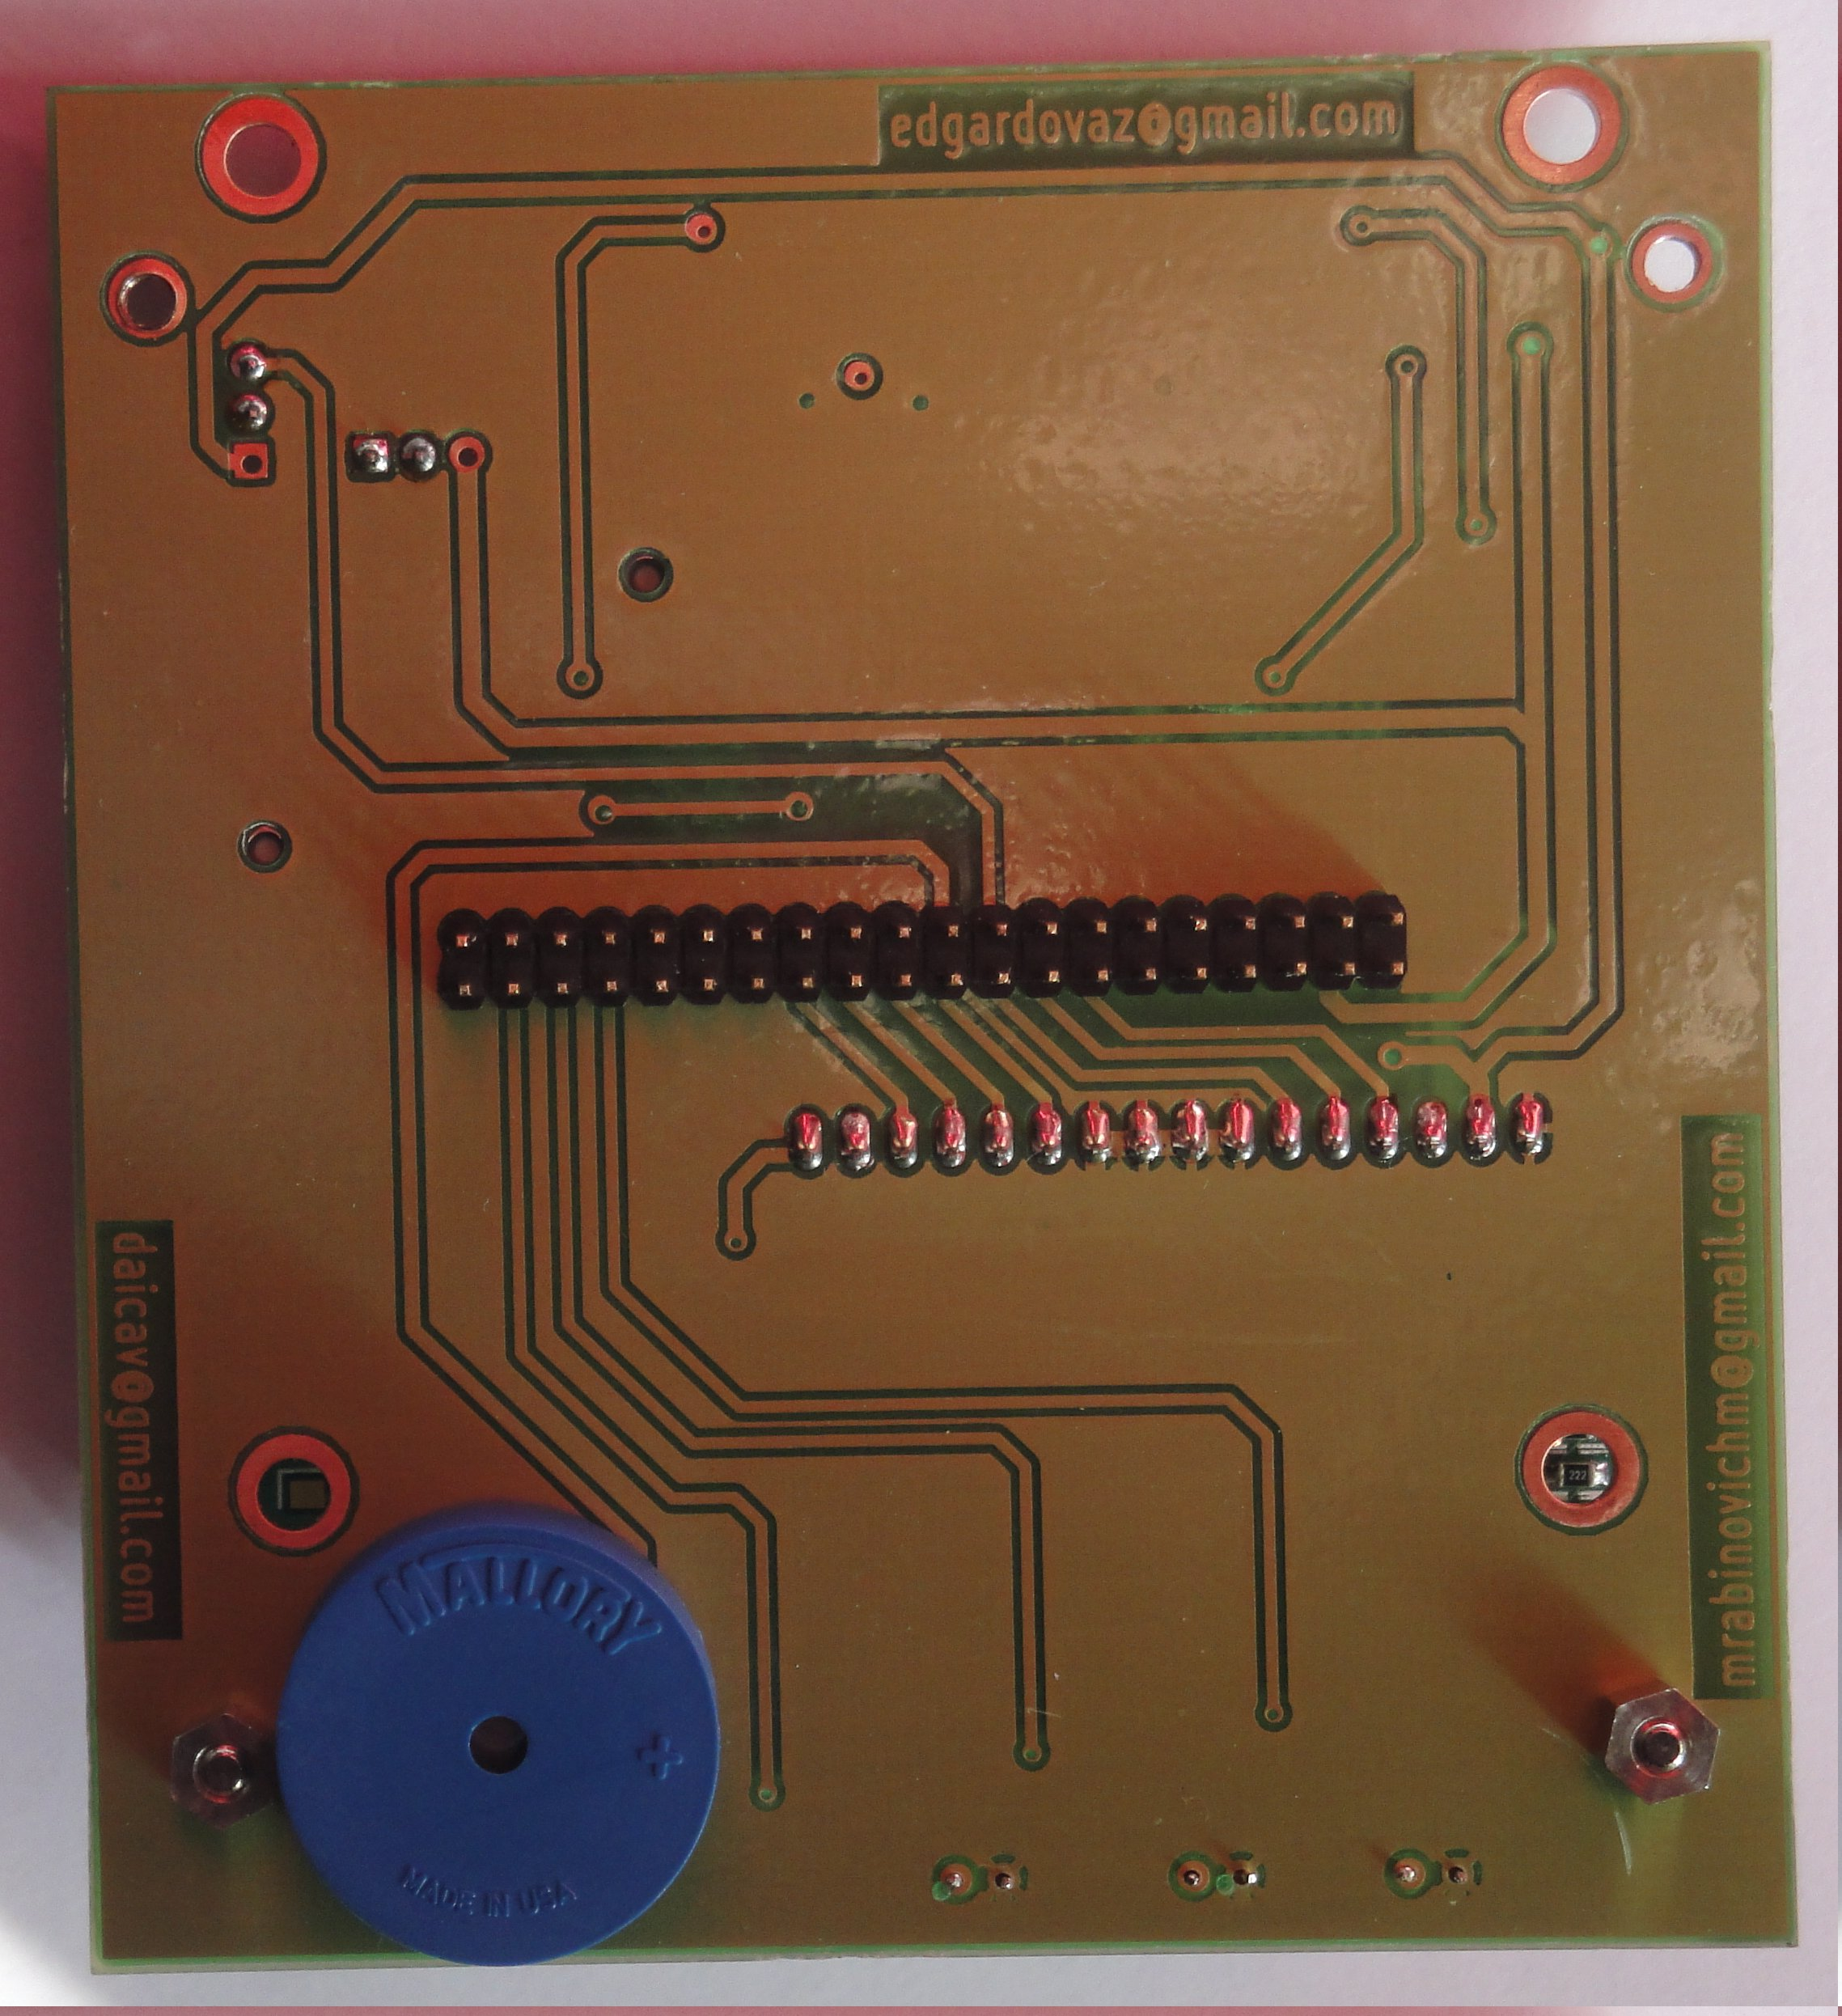
\includegraphics[scale=.033]{Imagenes/SCUI_b.jpg} }
	\end{figure}

	\begin{itemize}
		\item se integran en un mismo PCB
		
		\bigskip		
		\item no contiene ASICs

		\bigskip
		\item se diseñó y fabricó completamente
	\end{itemize}
\end{frame}

\begin{frame}
	\frametitle{RFID}
	Lector/escritor de tarjetas RFID:
	\begin{figure}
		\subfigure{
  			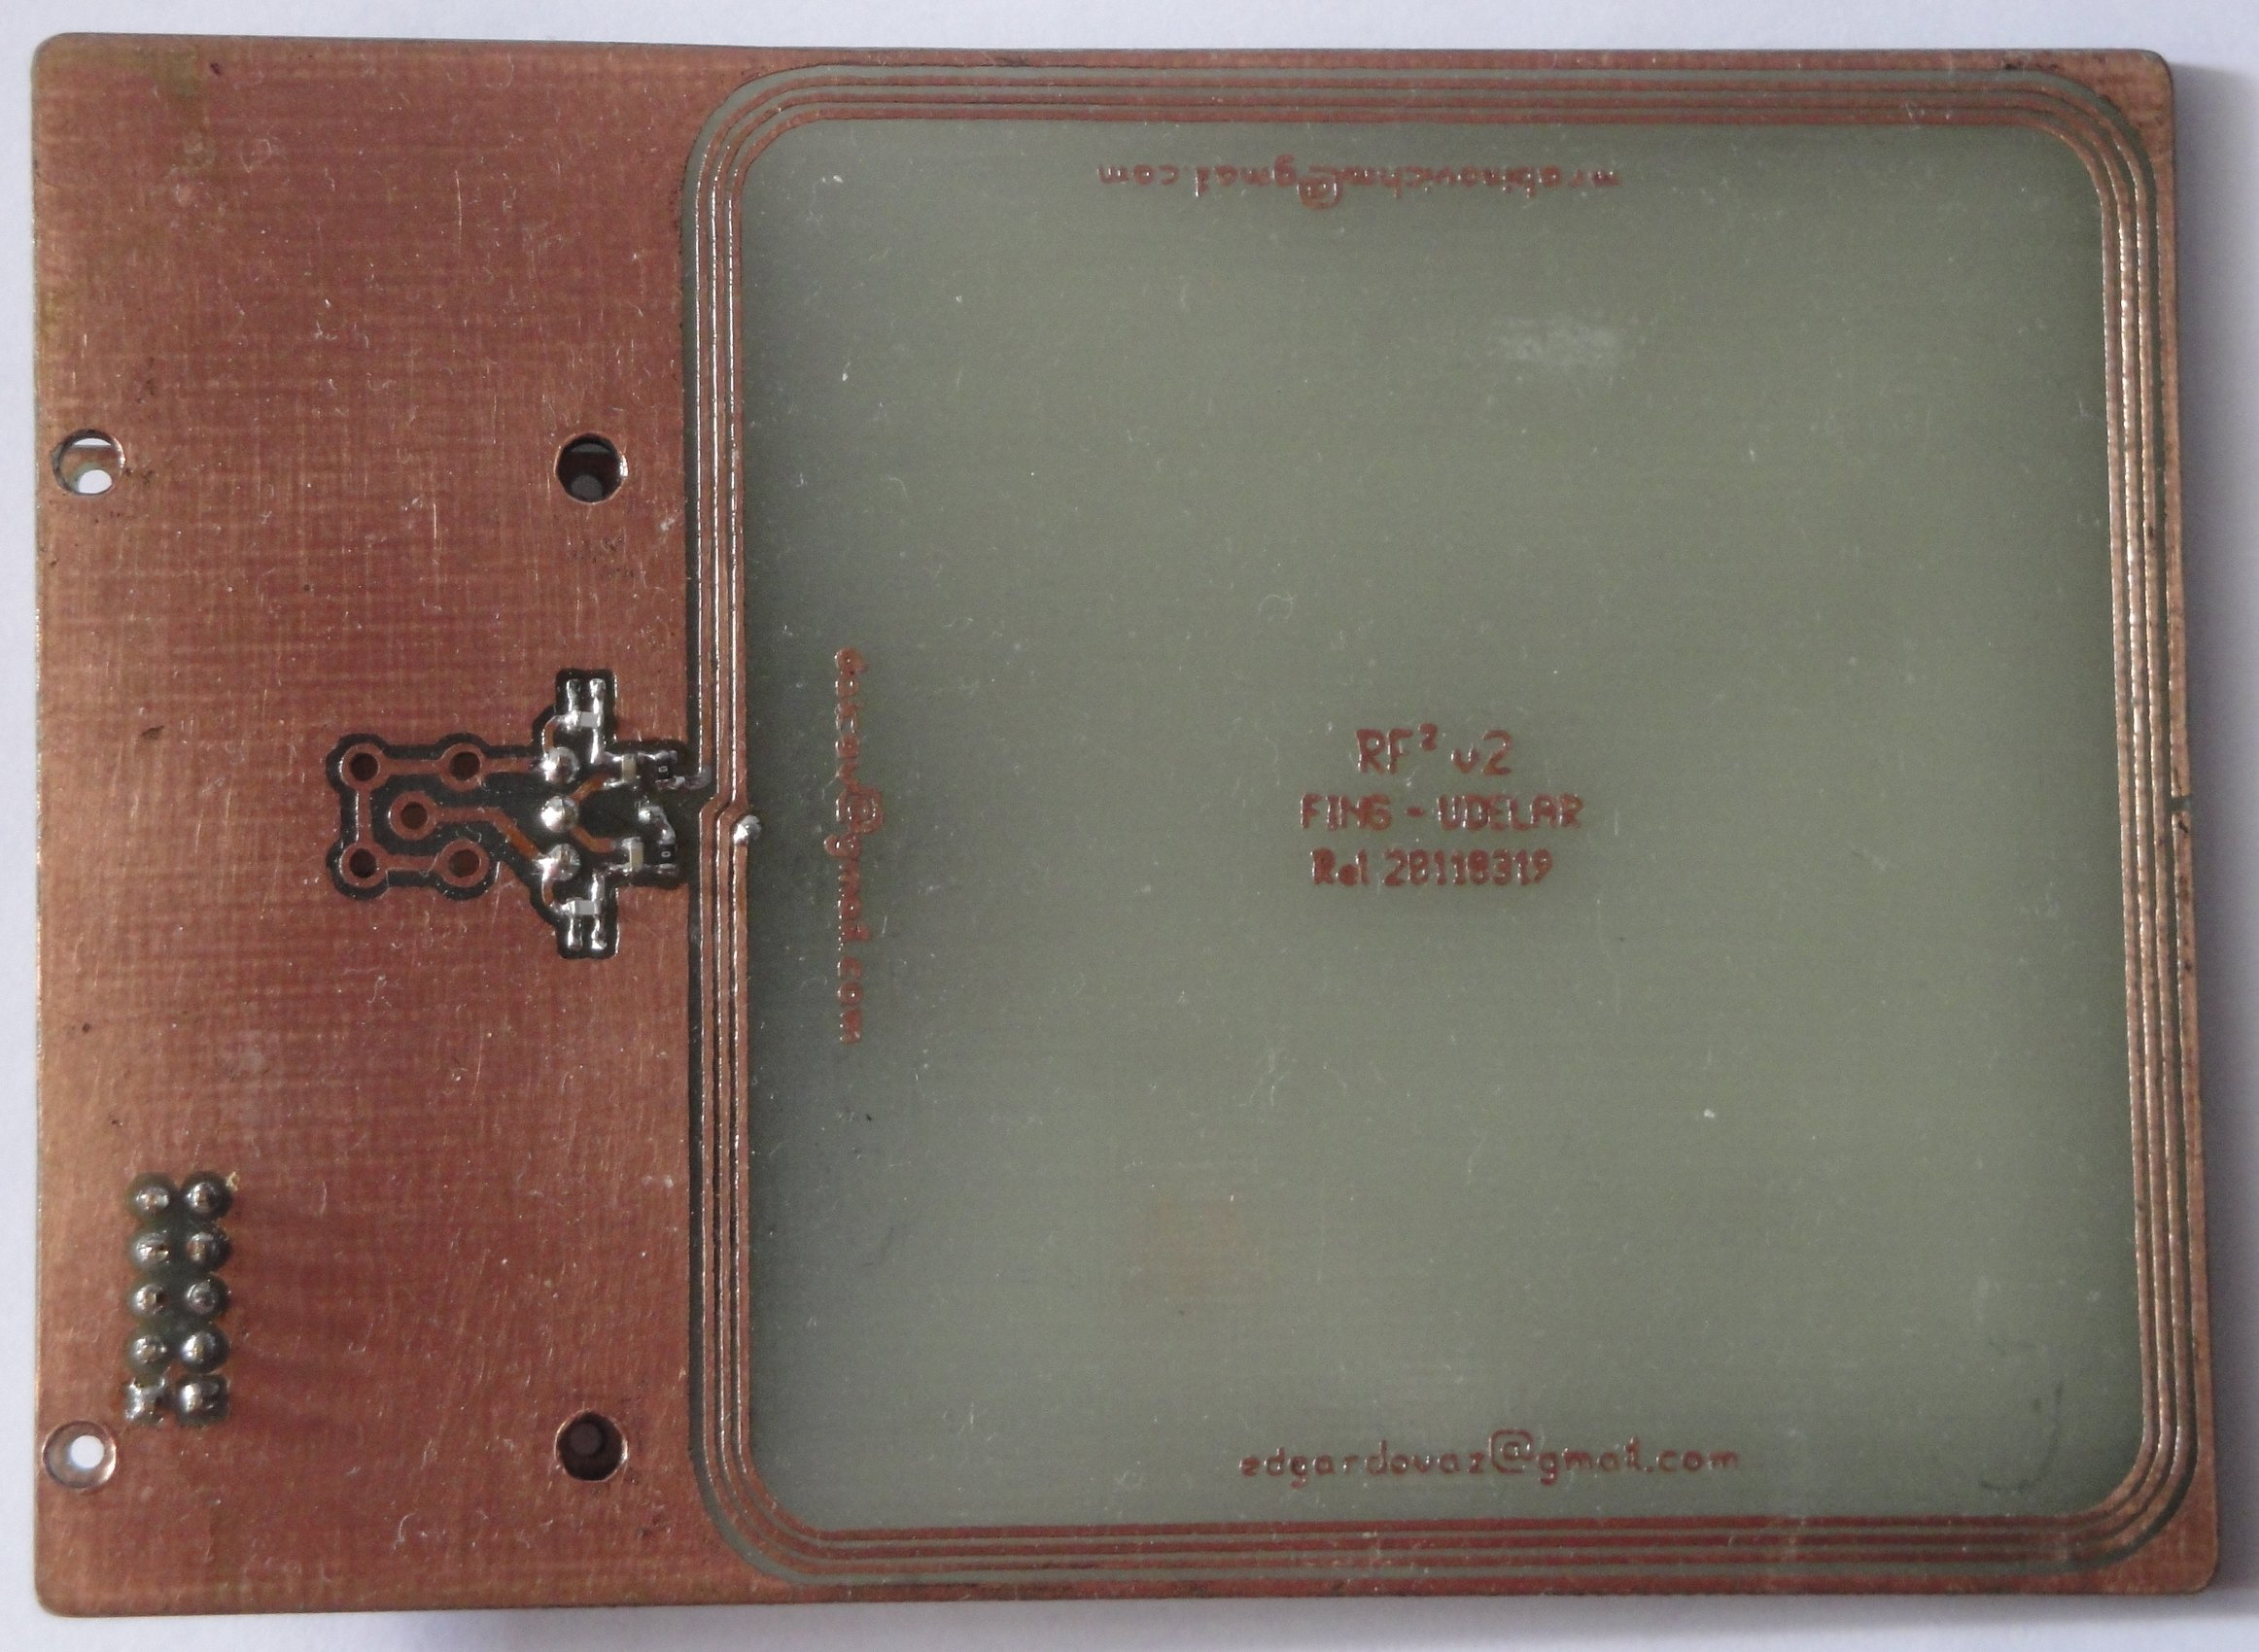
\includegraphics[scale=.04]{Imagenes/ant_f.jpg} } 
		\subfigure{ 
			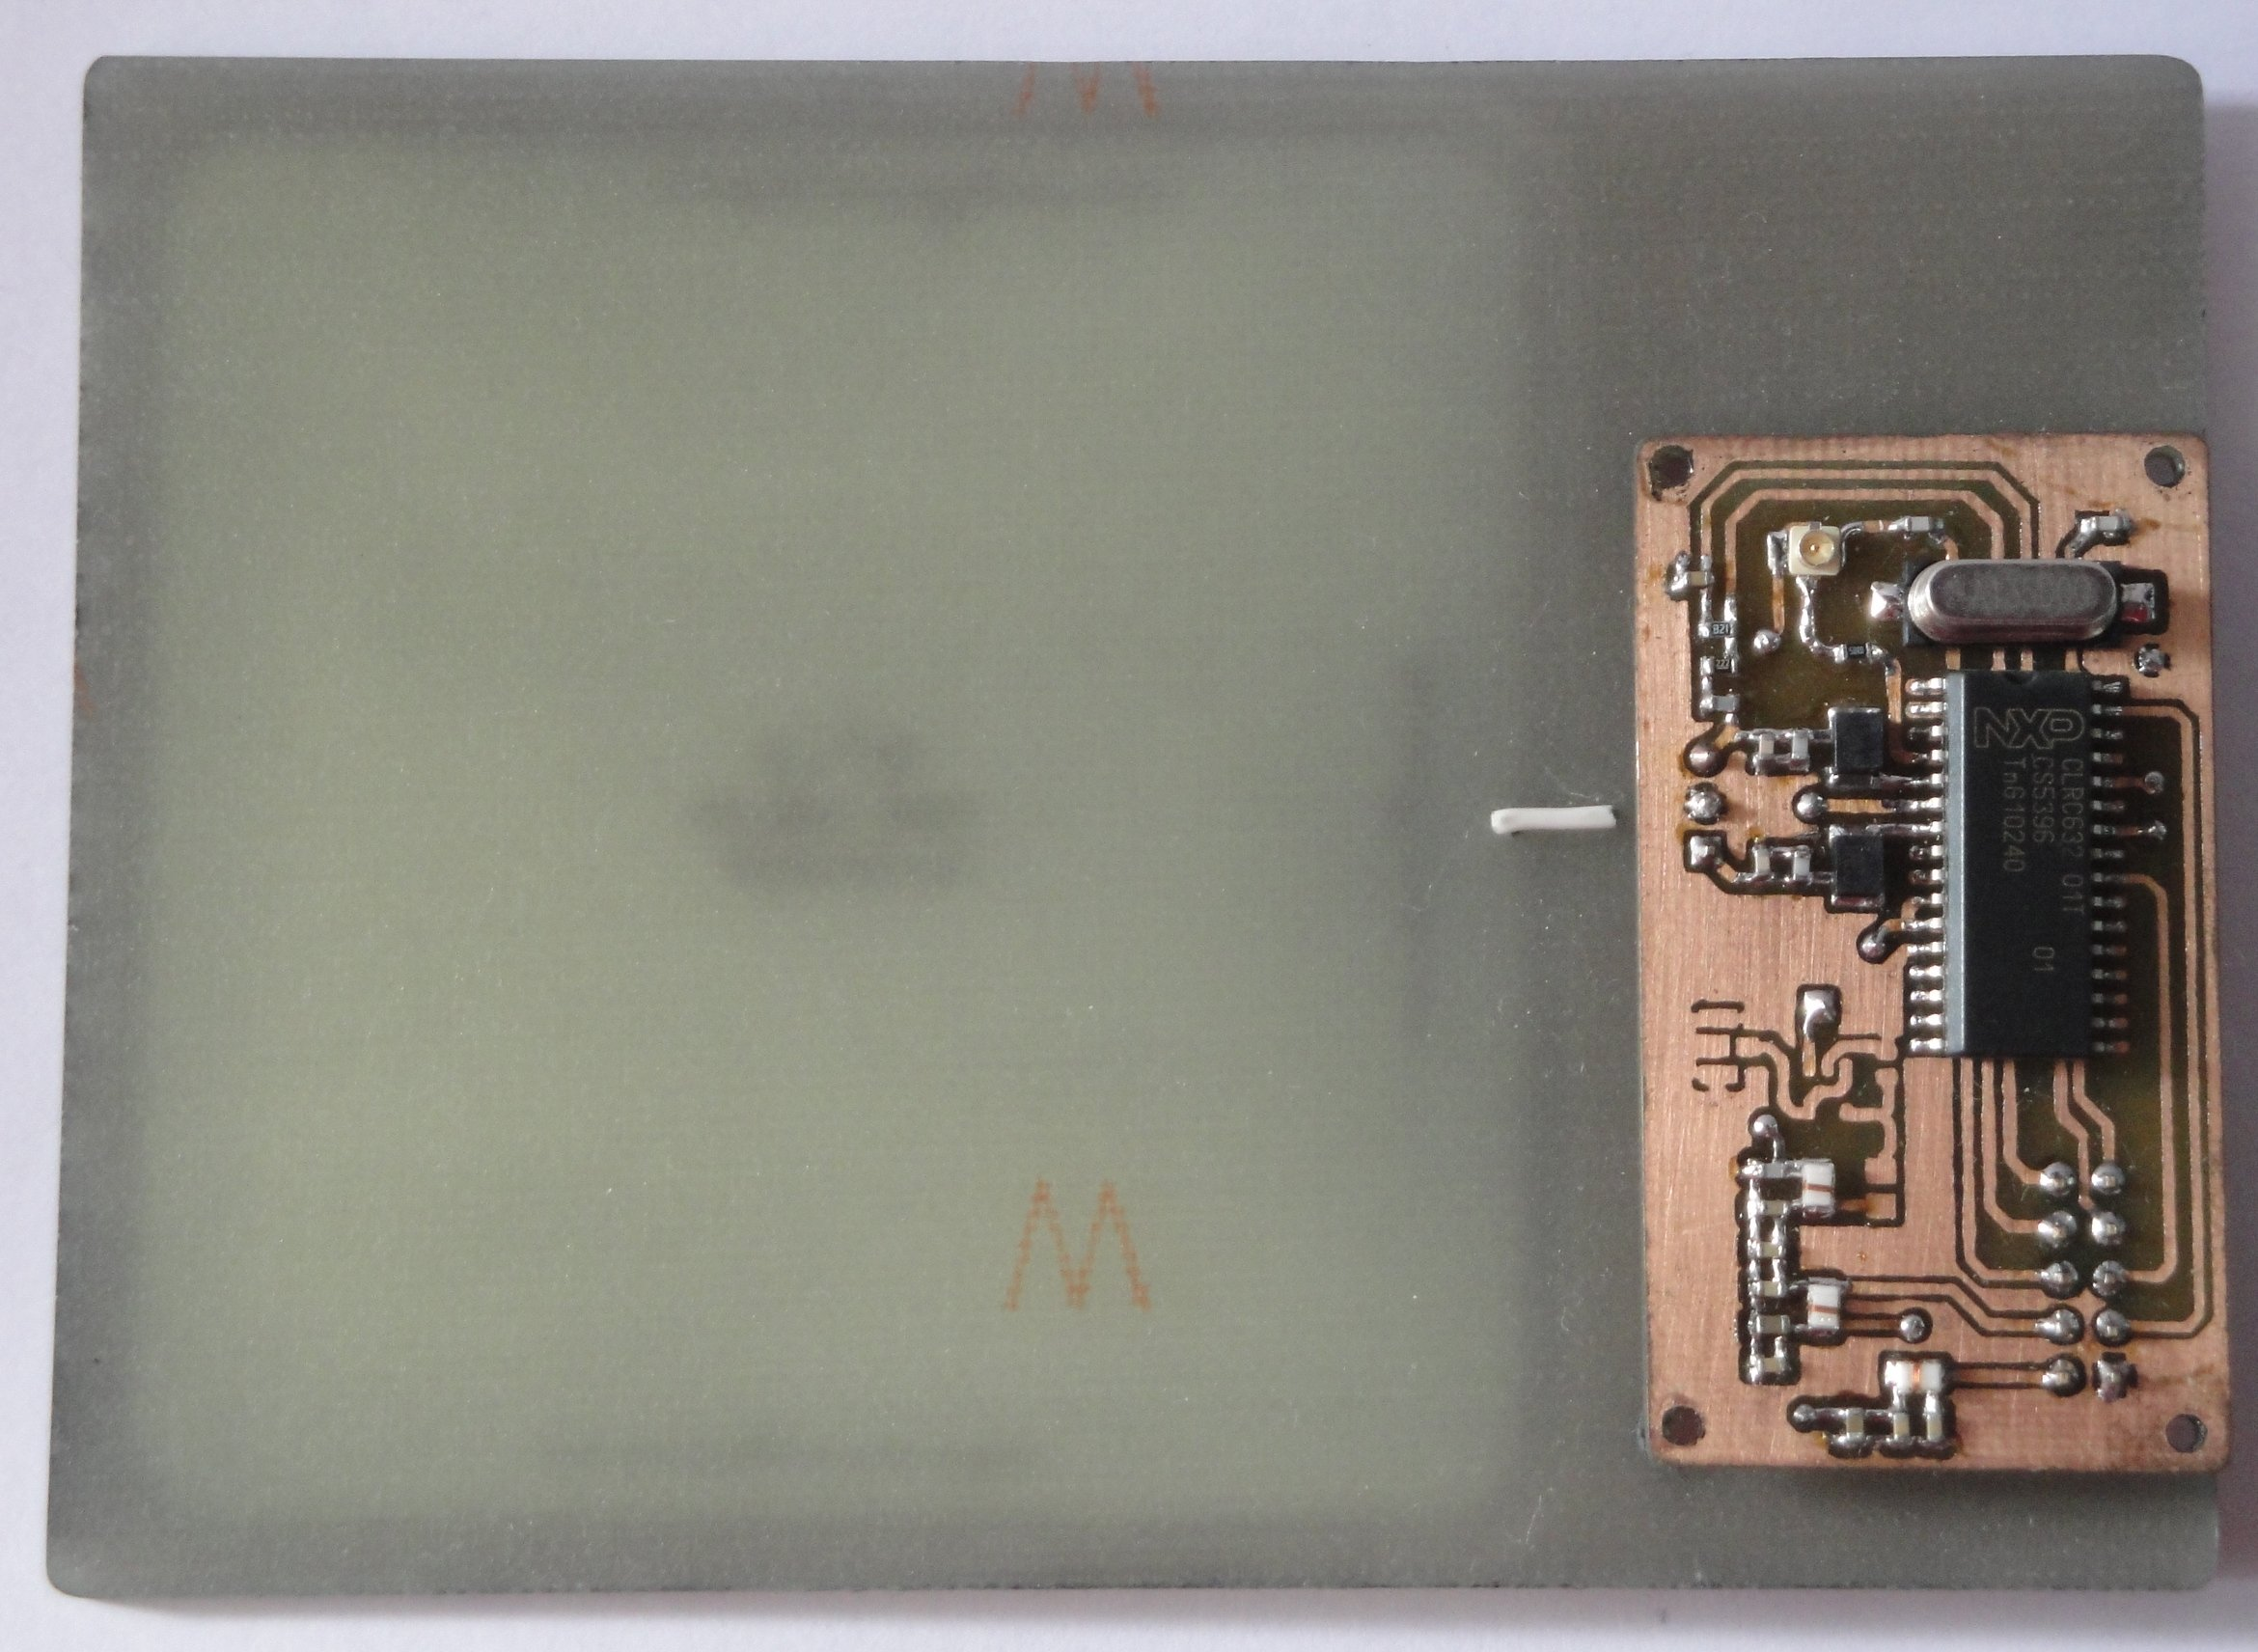
\includegraphics[scale=.04]{Imagenes/ant_b.jpg} }
	\end{figure}

	\begin{itemize}
		\item PCB a 2 capas

		\bigskip
		\item tarjetas sin contacto (13,56MHz)

		\bigskip
		\item CL RC632 se encarga del protocolo para las tarjetas (Mifare)

		\bigskip
		\item se diseñó y fabricó completamente
	\end{itemize}
\end{frame}

\begin{frame}
	\frametitle{Descripción general de funcionamiento}
	\textcolor{red}{acá va el diagrama con las partes? (i+12 de lo planeado)}
\end{frame}	
	
%%\section{Software}
%\subsection{Diagrama de flujo simplificado}
\begin{frame}
	\frametitle{Diagrama de flujo simplificado}
	\textcolor{red}{acá va el diagrama de flujo :)}
\end{frame}		
	
%\subsection{Software empleado}
\begin{frame}
	\frametitle{Software}
	\begin{itemize}
		\item Sistema Operativo GNU/Linux

		\bigskip
		\item Distribución Angström

		\bigskip
		\item Herramientas de desarrollo: 
		\begin{itemize} 
			\item OpenEmbedded-Bitbake 
			\item Narcissus 
		\end{itemize}
	\end{itemize}
\end{frame}		

%\subsection{Bibliotecas}
\begin{frame}
	\frametitle{Bibliotecas}
	\begin{itemize}
		\item librfid, editada (herramienta librfid-tool contiene el programa principal)

		\bigskip
		\item libgpio, completamente implementada

		\bigskip
		\item liblcd, editada (completamente implementada en 2009)

		\bigskip
		\item libpcsclite
	\end{itemize}

\textcolor{red}{diagrama de capas de software}
\end{frame}

\begin{frame}
	\frametitle{Bibliotecas}
	\textcolor{red}{diagrama de capas de software librfid-tool}

	Funciones de utilidad de la herramienta librfid-tool:
	\begin{itemize}
		\item lectura de tarjeta completa

		\bigskip
		\item lectura de un sector específico

		\bigskip
		\item escritura de un sector específico
	\end{itemize}
\end{frame}

%%\section{Ensayos}
\begin{frame}
	\frametitle{SBC}
	\begin{columns}
		\begin{column}{8cm}	
			\begin{itemize}
				\item Hawkboard	
				\begin{itemize}
					\item errores en el booteo
					\item por momentos se "tranca"
				\end{itemize}

				\bigskip			
				\item Beagleboard
				\begin{itemize}
					\item multiplexado de pines con u-boot, imposible
					\item[ ] Solución: hacerlo por kernel
					\item problemas con memoria SD
					\item[ ] Solución: sustituirla, tenía bloques rotos
				\end{itemize}
			\end{itemize}
		\end{column}	
		\begin{column}{3cm}		
			\begin{center}
				
\includegraphics[scale=.3]{Imagenes/preg.jpg}
			\end{center}
		\end{column}
	\end{columns}
\end{frame}

\begin{frame}
	\frametitle{SCUI}
	\begin{itemize}
		\item UI - Interfaz de usuario
		\begin{itemize}		
			\item errores de impresión en el display
			\item[ ] Solución: modificar código pasando ASCII
	\end{itemize}

	\bigskip
	\item SC - lector/escritor de tarjetas de contacto
		\begin{itemize}
			\item oscilador no funciona
			\item[ ] Solución: cambio de oscilador a frecuencia particular no antojadiza

			\bigskip
			\item PCB VLT causó problemas en la recepción
			\item[ ] Solución: cambiar resistencia en el lector/escritor
		\end{itemize}	
	\end{itemize}
\end{frame}

\begin{frame}
	\frametitle{RFID}
	\begin{columns}
		\begin{column}{10cm}
			\begin{itemize}
				\item testeo hw en un rabbit por falta de SBC
		
				\bigskip
				\item la antena no genera campo magnético
				\item[ ] Solución: bobina externa al PCB

				\bigskip		
				\item error en el circuito de matcheo 
				\item[ ] Solución: analizador de redes, cambio de capacitores
		
				\bigskip
				\item problemas al leer tarjetas
				\item[ ] Solución: cambio de f$_{clk}$ del puerto de comunicación, único cambio en 									 biblioteca librfid
		
				\bigskip
				\item varias modificaciones en herramienta librfid-tool
			\end{itemize}
		\end{column}
		
		\begin{column}{1.5cm}
%			\begin{center}
				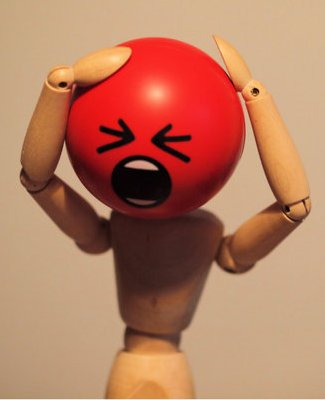
\includegraphics[scale=.6]{Imagenes/no.jpg}
%			\end{center}
		\end{column}
	\end{columns}
\end{frame}

%%\section{Costos}
\begin{frame}
	\frametitle{Costos}
	\begin{block}{Presupuesto}
		Se planificó un presupuesto total de U\$S1500, se gastaron alrededor de U\$S1400.
	\end{block}

	\begin{itemize}
		\item costos del proyecto sin mano de obra, excepto para PCBs comprados

		\bigskip
		\item PCBs en China a mitad de precio

		\bigskip
		\item se gastó menos de lo previsto, incluso con todos los gastos extra (SBC, VLT)
	\end{itemize}
\end{frame}	

\begin{frame}
	\frametitle{Tabla Comparativa}
	\textcolor{red}{acá va la tabla comparativa :p}
\end{frame}	

%\section{Mejoras}
\begin{frame}
	\frametitle{Mejoras posibles}
	\begin{itemize}
		\item terminar de integrar lector/escritor de tarjetas de contacto a PCSC-Lite

		\bigskip		
		\item realizar blindaje para la antena RFID
		
		\bigskip		
		\item fabricar carcasa, pasar a producción
		
		\bigskip		
		\item batería de respaldo, pequeño sistema para pocos minutos de autonomía
		
		\bigskip		
		\item migrar de SD a NAND Flash

		\bigskip		
		\item integrar todo a un único PCB
		
	\end{itemize}		
	\textcolor{red}{ver alguna otra opción existente en doc}
\end{frame}	


\begin{frame}
	\frametitle{Logros realizados}
	\begin{itemize}
		\item primer lector/escritor RFID 13,56MHz fabricado y diseñado en Uruguay

		\bigskip		
		\item prototipo multipropósito (sistema de transporte, control de acceso, marcas de personal)

		\bigskip		
		\item perseverancia pese al “cliente”
		
		\bigskip		
		\item sistema 24/7 y autónomo
		
		\bigskip		
		\item cambio de SBC en un momento adecuado
		
		\bigskip		
		\item PCB lector/escritor de tarjetas RFID a 2 capas

	\end{itemize}		
\end{frame}			

%\section{Conclusiones}
\begin{frame}
	\frametitle{Conclusiones y Reflexiones}
	
	\begin{columns}	
		\begin{column}{9cm}
			\begin{itemize}
				\item se logró el objetivo %
\includegraphics[scale=.2]{Imagenes/sinomas.jpg}

				\bigskip
				\item se destaca el trabajo en equipo

				\bigskip
				\item generación de conocimiento

				\bigskip
				\item solución académica a un problema real

				\bigskip
				\item las empresas debieran buscar soluciones tecnológicas a través de la Universidad como referente de conocimiento. No buscar y comprar siempre hecho afuera, que quede el conocimiento en el país.
			\end{itemize}		
		\end{column}
		
		\begin{column}{2cm}
			\begin{center}
				
\includegraphics[scale=.2]{Imagenes/sinomas.jpg}

				\bigskip
				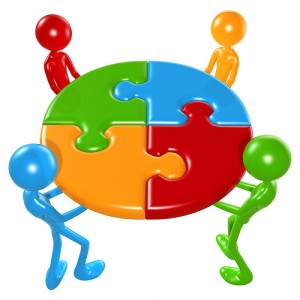
\includegraphics[scale=.2]{Imagenes/EQUIPO.jpg} %equipo.3


				\bigskip
				
\includegraphics[scale=.3]{Imagenes/udelar.jpg}				
			\end{center}
		\end{column}
	\end{columns}
\end{frame}			
%\subsection{Campos de aplicación}
%\begin{frame}
%	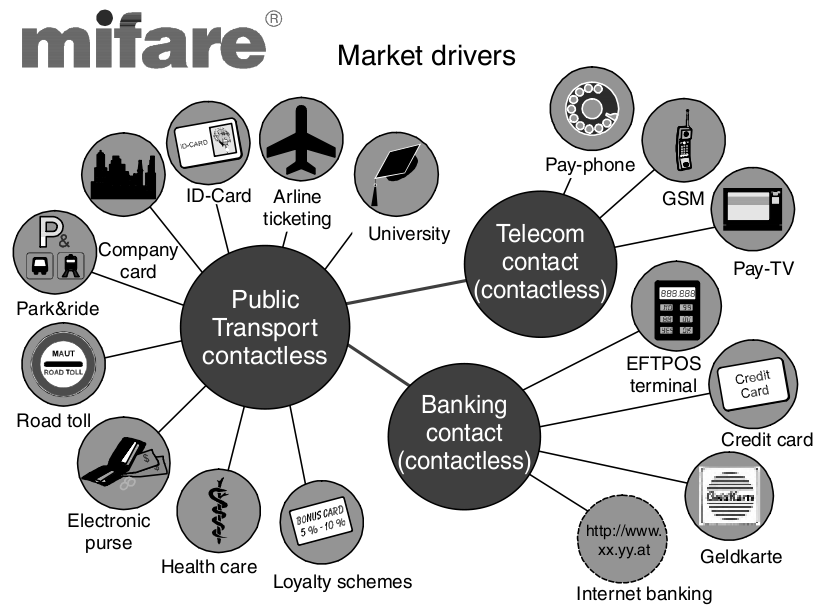
\includegraphics[scale=.4]{Imagenes/aplicaciones.png}
%\end{frame}


%%%%%%%%%%%

%\section{Preguntas}
\begin{frame}
	\frametitle{Preguntas}
	\begin{center}
		\bigskip		
		
\includegraphics[scale=.25]{Imagenes/preguntas.jpg}
	\end{center}
\end{frame}

\end{document} 